\documentclass{standalone}
\usepackage[utf8]{inputenc}
\usepackage{pgfplots}
\usetikzlibrary{decorations.pathreplacing,calligraphy}

\pgfplotsset{compat=1.3, xlabel=$t$,ylabel=$P$,zlabel=$z$}

\begin{document}
    \pgfplotsset{width=9cm}
    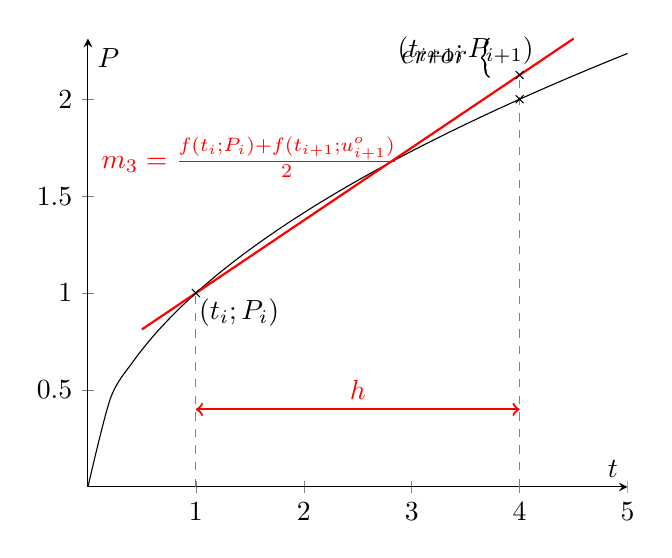
\begin{tikzpicture}
        \begin{axis}[legend cell align=left,
            legend pos=outer north east,ymin=0,xmin=0,
            domain=0:5,clip=false,axis lines=middle]
            \addplot[smooth,color=black] {sqrt(x)};
            \addplot [mark=none,  red,  thick] coordinates { (0.5,0.8125) (4.5,2.3125)};
            \addplot [mark=none,  color=gray,  dashed] coordinates { (1,0) (1,1)}; %punt1
            \addplot [mark=none,  color=gray,  dashed] coordinates { (4,0) (4,2.125)}; %punt2
            \node at (axis cs:1.5,1.7) [red] {$m_3=\frac{f(t_i; P_i)+f(t_{i+1}; u^o_{i+1})}{2}$};
            \addplot [mark=x] coordinates{(1,1)}; %ti cross
            \node at (axis cs:1.4,0.9) {$(t_i; P_i)$}; %ti name
            \addplot [mark=x] coordinates{(4,2.125)}; %ti+1 cross
            \node at (axis cs:3.5,2.25) {$(t_{i+1}; P_{i+1})$}; %ti+1 name
            \addplot [mark=x] coordinates{(4,2)}; %P(ti+1) cross
        %    \node at (axis cs:4.8,1.9) {$(t_{i+1}; P(t_{i+1}))$}; %P(ti+1) name
            \addplot [<->, red, thick] coordinates{ (1,0.4) (4,0.4) } node[midway, above]{$h$};
        \end{axis}
                    %
    \begin{scope}[decoration={calligraphic brace,amplitude=3pt}]
        \draw[thick,decorate] (5.1,5.2) -- (5.1,5.7)
         node[midway,left=1ex]{$error$};
        \end{scope}
    \end{tikzpicture}
\end{document}